\section{Qualitative Analysis}

	\normalsize
	{
		There are many software quality models that have been formulated for the determination of quality improvement and analysis.  
		It's important to understand that when doing a qualitative analysis that ``all models are flawed, but some are useful''.
		In my undergraduate learning a software quality model was undertaken were I learned about Software Process Improvement(SPI)
		as well as some of the models available for this process.  
		\newline
		\newline
		A Taxonomy to Compare software process improvement(SPI) Frameworks by Christian Printzell Halvorsen and Reidar Conradi can be used in the 
		determination of the suitable software process improvement(SPI) framework for an organisation, however this from 
		an under graduate perspective, qualitative aspects required in the field are realistically unachievable 
		such as Geographic origin/spread, scientific origin, development/stability or Popularity.  
		\newline
		\newline
		Similarly this issue arose in choosing a qualitative analysis model and as such the choice for the ISO/IEC 9126
		for the evaluation of software quality was accepted due to the high level nature of the model.
		\newline
		\newline
		ISO/IEC 9126 outlines the following characteristics and from a quick glance the reader should be able to identify that this quality
		model has a lot of the ``ilities'' or non functional requirements.
		\newline
		
		\subsection{ISO/IEC 9126}
		
			\vspace{-5mm}
			\begin{multicols}{3}
		
				\begin{itemize}
					\item \textbf{Functionality}
						\begin{itemize}
							\item Suitability
							\item Accuracy
							\item Interoperability 
							\item Security
							\item Compliance
						\end{itemize}
						
					\item \textbf{Reliability}
						\begin{itemize}
							\item Maturity
							\item Fault Tolerance
							\item Recoverability 
							\item Compliance
						\end{itemize}	
						
					\columnbreak
						
					\item \textbf{Usability}
						\begin{itemize}
							\item Understandability
							\item Learnability
							\item Operability 
							\item Attractiveness
							\item Compliance
						\end{itemize}	
						
					\item \textbf{Efficiency}
						\begin{itemize}
							\item Time Behaviour
							\item Resource Utilisation
							\item Compliance 
						\end{itemize}	
					
					\columnbreak
						
					\item \textbf{Maintainability}
						\begin{itemize}
							\item Analysability
							\item Changeability
							\item Stability 
							\item Testability
							\item Compliance
						\end{itemize}	
						
					\item \textbf{Portability}
						\begin{itemize}
							\item Adaptability
							\item Installability
							\item Co-Existence 
							\item Replaceability
							\item Compliance
						\end{itemize}	
						
				\end{itemize}	
				
			\end{multicols}
	}	

\newpage	

	\large{\bfseries{Functionality}}
	\vspace{2mm}
	
	\normalsize
	{
		The implementation met all the requirements set out in the objectives and as such is suitability functional.
		As security was not taken into account when under development, some changes have to be made in order to 
		comply with the ISO/IEC 9126 model.  Integration with site authentication mechanisms such as Kerberos (Public Key Cryptography) or some other
		public key technology would be the next logical step to ensure security compliance.
		\newline	
	}				
	
	\large{\bfseries{Reliability}}	
	\vspace{2mm}

	\normalsize
	{
		Due the extensive testing during development most critical and bugs were identified and resolved and as a result
		the client server implementation as run for days consistently without any internal errors.
		Administrators who create modules will need to test their modules in a non live environment 
		to ensure the stability and fault tolerance of these modules.
		\newline	
	}				

	\large{\bfseries{Usability}}
	\vspace{2mm}

	\normalsize
	{
		The choice to implement the administrator interface using C\# and Windows Presentation Foundation (WPF)
		give greater accessibility to the non savvy administrators looking for an a bridge from the windows administration 
		environment to the Linux environment.  As such the administrator interface offers an attractable assessable means
		to accomplish greater learnability and understandability from a non Linux administrator.
		\newline	
	}

	\large{\bfseries{Efficiency}}
	\vspace{2mm}

	\normalsize
	{
		The client server implementation has the ability to serve 1000 requests and replies in an 8 second period.
		This is more than sufficient to handle a large network environment.  A trade off had to be made for the implementation
		in terms of portability and extensibility, in that Perl was chosen instead of per say C++.  
		As PERL is an interpreted language is does not have the same efficiency as a compiled language such as C++. 
		In a large scale network, administrators would not rely on any one server to service all these requests and in 
		this case a round robin in the domain name service is set up to help load balance requests on servers.
		In this case the scalability of the implementation supersedes and negative efficiency factors.
		\newline	
	}
	
	\large{\bfseries{Maintainability}}
	\vspace{2mm}

	\normalsize
	{
		As per a modular design you would expect to see no coupling of the components, this is illustrated by the dependency graph in
		Fig. \ref{fig:DependancyMethodsRelationshipDiagram} \& \ref{fig:DependancyTypesRelationshipDiagram}.  
		This offers developers to ship updates to individual components.  
		\newline	
		\newline
		
		\begin{figurehere}
			\centering
			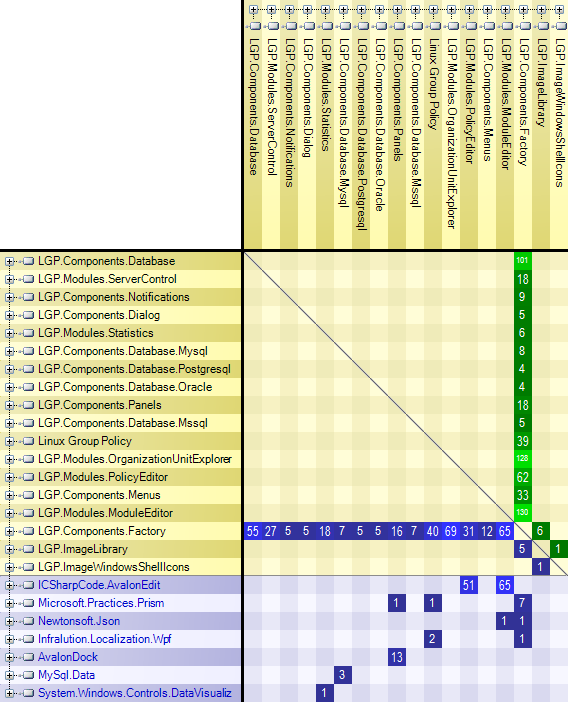
\includegraphics[scale=0.85]{pages/chapter4/figures/dependancyMatrixMethods.png}
			\caption{Dependency Methods Relationship Diagram}
			\label{fig:DependancyMethodsRelationshipDiagram}
		\end{figurehere}
		
		\vspace{5mm}
		Fig. \ref{fig:DependancyMethodsRelationshipDiagram} shows the method relationship or method call coupling between each 
		of the composite components, while Fig. \ref{fig:DependancyTypesRelationshipDiagram} shows the type relationship or 
		coupling between each of the composite components.  
		\newline
		\newline
		
		\begin{figurehere}
			\centering
			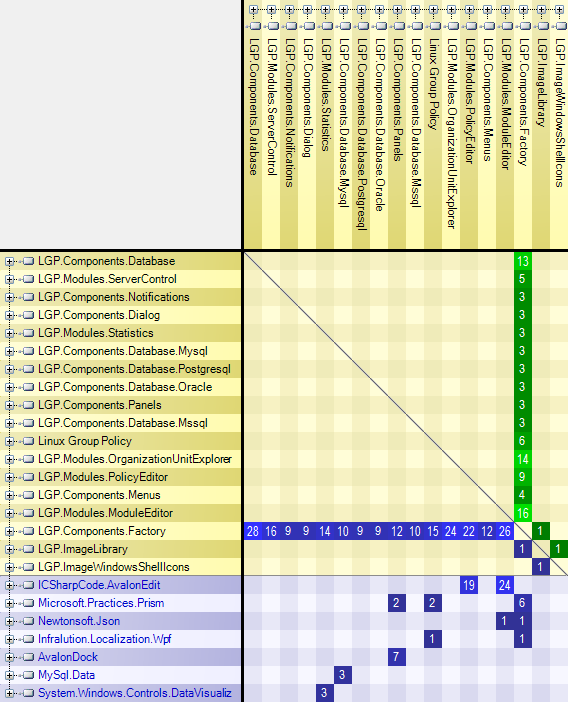
\includegraphics[scale=0.85]{pages/chapter4/figures/dependancyMatrixTypes.png}
			\caption{Dependency Types Relationship Diagram}
			\label{fig:DependancyTypesRelationshipDiagram}
		\end{figurehere}
		
		\vspace{5mm}
		From these diagrams it is clearly indicated that there is no coupling of the implementation's 
		composite components and as previously stated this allows me to develop a composite component further and 
		ship this update separately if necessary.
		\newline
	}			

	\large{\bfseries{Portability}}
	\vspace{2mm}
	
	\normalsize
	{
		The client server product is based upon Perl for maximum portability.  Since all major distributions ship with Perl as default 
		this ensure maximum portability.  Further more the Comprehensive Perl Archive Network (CPAN) is accessible by Perl as default 
		and allows administrators to update and install Perl modules relatively easily.  
		\newline
		\newline
		Vendor specific PERL implementations such as ActiveState also provide this functionality of updating modules 
		on the fly.  As there is no compilation needed the installability of the 
		client is purely dependant on the existence of Perl on the particular distribution.
		\newline
		\newline
		Due to the modular nature of the client and the associated interpreter, the replaceability and adaptability of the client server
		implementation is a factor of the administrators ability to create modular tailored for the organisation's environment.
		\newline
		\newline
		In the long run, modules would be kept in a Comprehensive Perl Archive Network (CPAN) fashion on an external server.
		Administrators mere only search this online repository for modules that can be integrated into their environment giving maximum 
		replaceability and adaptability.
		\newline					
	}
	
	\large{\bfseries{Project Management}}
	\vspace{2mm}
	
	\normalsize{\textit
	{
		PMBoK describes Project management as the application of knowledge, skills, tools, and techniques
		to project activities in order to meet or exceed stakeholder needs and expectations from a project. 
		\newline
		\newline
		Meeting or exceeding stakeholder needs and expectations invariably involves balancing competing demands among Scope, time, cost \& quality. - (PMBoK)
		\newline
	}}
				
	\normalsize
	{
		In this section we will look at the two excerpts from project management relevant to the successful completion of this product \& the report.
		\begin{itemize}				
			\item \textbf{Scope, time, cost, and quality}
			\item \textbf{Change control}
		\end{itemize}	
		\vspace{3mm}
	}
		
	\large{\bfseries{Scope, Time, Cost \& Quality}}
	
	
	
	
	
	\vspace{-3mm}
	\begin{multicols}{2}
	  
		\normalsize
		{
			\textbf{Scope} : 
			\textit
			{
				\begin{itemize}
					\item Initiation - committing the organisation to begin the next phase of the project
					\item Scope Planning - developing a written scope statement as the basis for future project decisions
					\item Scope Definition - subdividing the major project deliverables into smaller, more manageable components
				\end{itemize}	
			}	
		}
			
		\columnbreak
								
		\begin{figurehere}
			\centering
			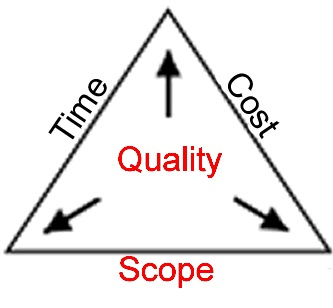
\includegraphics[scale=0.5]{pages/chapter4/figures/scope.jpg}
			\caption{Scope}
			\label{fig:QScope}
		\end{figurehere}
			
	\end{multicols}
			
	\vspace{-10mm}
	\normalsize
	{		
		\textit
		{
			\begin{itemize}
				\item Scope Verification - formalizing acceptance of the project scope								
				\item Scope Change Control - controlling changes to project scope
			\end{itemize}
		}
		- (PMBoK)
		\newline

		The decision to commit to a project is highly dependant on the scope and associated skills.
		As the project was adequately defined, planned and verified this negated any possible side effect on time and cost.
		\newline
	}
			
		
		
		
		
	\begin{multicols}{2}
  
		\normalsize
		{
			\textbf{Time} :
			\textit
			{
				\begin{itemize}
					\item Activity Definition - identifying the specific activities that must be per-formed to produce the various project deliverables
					\item Activity Sequencing - identifying and documenting interactivity dependencies
					\item Activity Duration Estimating - estimating the number of work periods which will be needed to complete individual activities
				\end{itemize}	
			}			
		}
			
		\columnbreak
								
		\begin{figurehere}
			\centering
			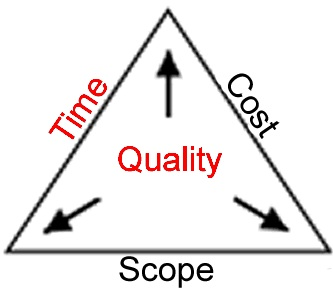
\includegraphics[scale=0.5]{pages/chapter4/figures/time.jpg}
			\caption{Time}
			\label{fig:QTime}
		\end{figurehere}
		
	\end{multicols}
		
	\vspace{-10mm}
	\normalsize
	{		
		\textit
		{
			\begin{itemize}
				\item Schedule Development - analyzing activity sequences, activity durations, and resource requirements to create the project schedule								
				\item Schedule Control - controlling changes to the project schedule
			\end{itemize}	
		}
		- (PMBoK)
		\newline

		Time is a major concern in final year projects and as such the decision to undertake the project was carefully 
		considered.  Of the 5 lecturers I spoke too, one of them said outright it would not be possible, another said it
		would be a PHD project, while three of the lecturers exhibited mixed reactions towards to project.
		\newline
		\newline
		The Gannt chart in Fig. \ref{fig:GanntChart} however help me to realize the project was feasible in the allotted 
		time frame.  I was confident in my skills and believed through previous experience that the project was very feasible;
		Although a little more than I wanted to do in order to achieve a successful result.
		\newline
	}
	
	
	\vspace{-5mm}
	\begin{multicols}{2}
  
		\normalsize
		{
			\textbf{Cost} :
			\textit
			{
				\begin{itemize}
					\item Resource Planning - determining what resources (people, equipment, mate-rials) and what quantities of each should be used to perform project activities
					\item Cost Estimating - developing an approximation (estimate) of the costs of the resources needed to complete project activities
					\item Cost Budgeting - allocating the overall cost estimate to individual work items
				\end{itemize}
			}	
		}
			
		\columnbreak
								
		\begin{figurehere}
			\centering
			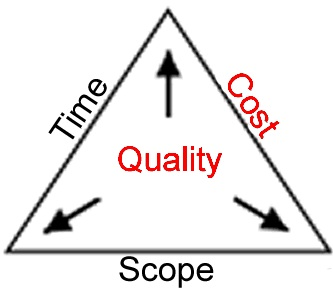
\includegraphics[scale=0.5]{pages/chapter4/figures/cost.jpg}
			\caption{Cost}
			\label{fig:QCost}
		\end{figurehere}
		
	\end{multicols}
	
	\vspace{-10mm}
	\normalsize
	{	
		\textit
		{
			\begin{itemize}
				\item Cost Control - controlling changes to the project budget			
			\end{itemize}
		}
		- (PMBoK)
		\newline
		
		The cost factor for final year projects I believe has two aspects.  Unlike the monetary aspects of commercial software,
		final year projects have to be balanced in-line with other work in other subjects.  For the first semester of 4th year
		I achieved a semester grade of 3.6.  So the cost was relatively low in this regard.  The second cost for me was hair
		loss, i gave it about 25\%, I think I lost around 10\%, so it has been a ``win win'' in terms of cost so far!
	}
		
		
		
		
		
	\begin{multicols}{2}
  
		\normalsize
		{
			\textbf{Quality} : 
			\textit
			{
				\begin{itemize}
					\item Quality Planning - identifying which quality standards are relevant to the project and determining how to satisfy them
					\item Quality Assurance - evaluating overall project performance on a regular basis to provide confidence that the project will satisfy the relevant quality standards
				\end{itemize}		
			}
		}
			
		\columnbreak
								
		\begin{figurehere}
			\centering
			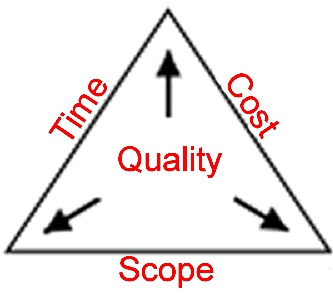
\includegraphics[scale=0.5]{pages/chapter4/figures/quality.jpg}
			\vspace{-3mm}
			\caption{Quality}
			\label{fig:QQuality}
		\end{figurehere}	
		
	\end{multicols}
	
	\vspace{-10mm}
	\normalsize
	{	
		\textit
		{
			\begin{itemize}
				\item Quality Planning - identifying which quality standards are relevant to the project and determining how to satisfy them
				\item Quality Assurance - evaluating overall project performance on a regular basis to provide confidence that the project will satisfy the relevant quality standards
			\end{itemize}		
		}
		- (PMBoK)
		\newline
		\newline
		The result when balancing from the outcomes of scope achievement, cost and time management determine the quality 
		of the project in project management.  As all the requirements of the scope were met, it was achieved ahead of time and 
		the cost was low, the quality of the project and its outcomes are deemed to be high quality!
		\newline
	}
				
		
	\begin{figurehere}
		\centering
		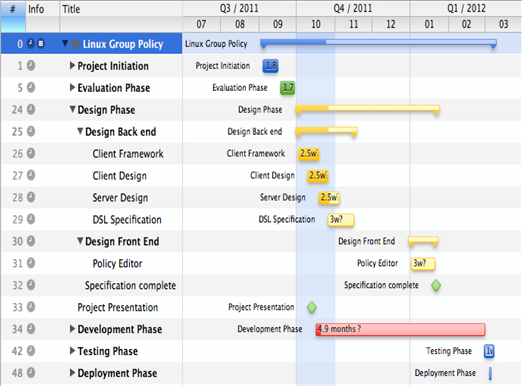
\includegraphics[scale=0.9]{pages/chapter4/figures/timeline.png}
		\caption{Gannt Chart}
		\label{fig:GanntChart}
	\end{figurehere}		
	
\newpage
	
	\subsection{Change Control}
	
		\normalsize
		{
			As the project manager is was my job to actively manage change control.  My supervisor
			tried a few times to change some of the requirements for which I was in favour and in some cases against.
			I knew the time, cost and scope of what had to be done and in most cases I rejected the changes put forth.
			\newline
			\newline
			Some projects have difficulties due to project managers accepting any and all change requests
			resulting in disillusioned, lack of direction development.  I was aware of this from previous experience
			and from the learning outcomes of the Project Management module I had done previously.
			\newline
			\newline
			The choice for me when accepting a change, is generally quiet simple and although may seem like the ``lazy''
			approach, it generally results in a favourable outcome.  Only minor changes would be accepted and they would result 
			in less scope.  The reason for this is based upon, how much development needs to change, and always to take less work,
			not more work.  Therefore if a change control results in less work in the future with an initial increase in work
			this is deemed acceptable.  This approach generally increases the overall quality of the software.
		}
	
		\vspace{5mm}
		\large{\bfseries{Version Control}}
				  
		\normalsize
		{
			We can see from the commit history in Fig. \ref{fig:commitscatterauthors} that the project had finished 
			in early February, approximately 2 weeks ahead of schedule.
			\newline
			\newline
			We can see the time-line of the development and that most of that work had been done in the winter holiday period.
			Fig. \ref{fig:locandchurn} shows the lines of code and churn level also indicating the increase
			of change during the lead up to the end of development.
			\newline
			\newline
			By using a version control software it allows me, the developer to provide the solution to 
			multiple customers at different stages of development.  By creating forks at specific versions allows
			me to fix bugs while still supporting the version that the customer has deployed.
			\newline
			\newline
			Eventually a subsequent merge of these forks would be done in order to reintegrate the software as a whole.
			Too many forks are difficult to manage and merge.
			\newline							
		}			
		
		\vspace{5mm}
		\begin{figurehere}
			\centering
			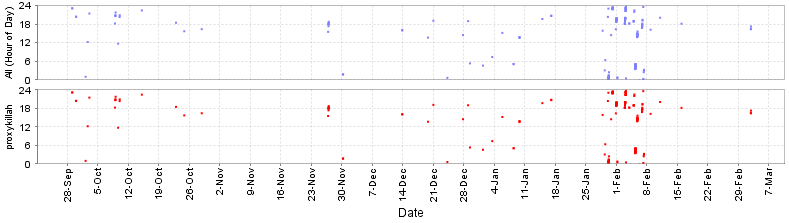
\includegraphics[scale=0.8]{pages/chapter4/figures/commitscatterauthors.png}
			\caption{Commit activity time line}
			\label{fig:commitscatterauthors}
		\end{figurehere}
		
		\vspace{5mm}
		\begin{figurehere}
			\centering
			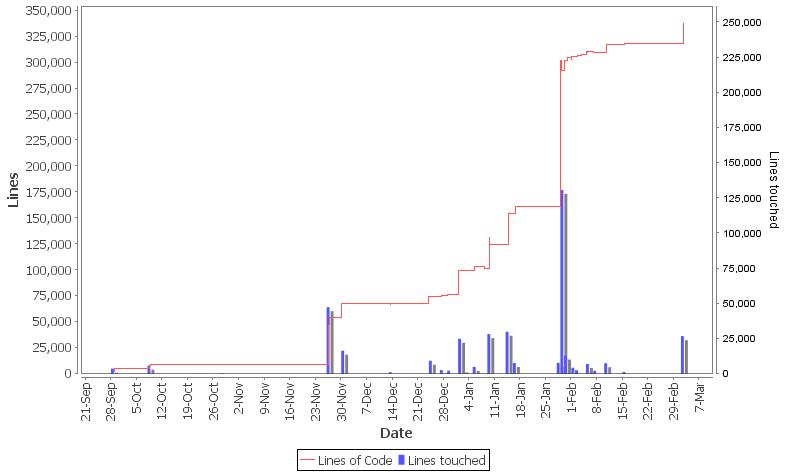
\includegraphics[scale=0.7]{pages/chapter4/figures/locandchurn.png}
			\caption{Lines of code \& churn level}
			\label{fig:locandchurn}
		\end{figurehere}		
		
		\vspace{5mm}
		\normalsize
		{
			I have also provided Fig. \ref{fig:activity_day} an analysis of the daily work
			\& Fig. \ref{fig:activity_time} the hourly rate of work to get a more discrete breakdown of the software 
			development life cycle.
			\newline					
		}
			
		\vspace{5mm}
		\begin{figurehere}
			\centering
			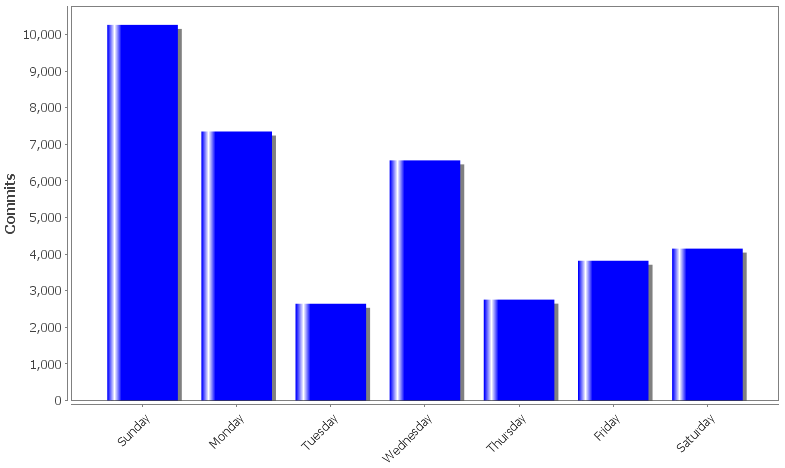
\includegraphics[scale=0.7]{pages/chapter4/figures/activity_day.png}
			\caption{Commit activity by day of the week}
			\label{fig:activity_day}
		\end{figurehere}
		
		\vspace{5mm}
		\begin{figurehere}
			\centering
			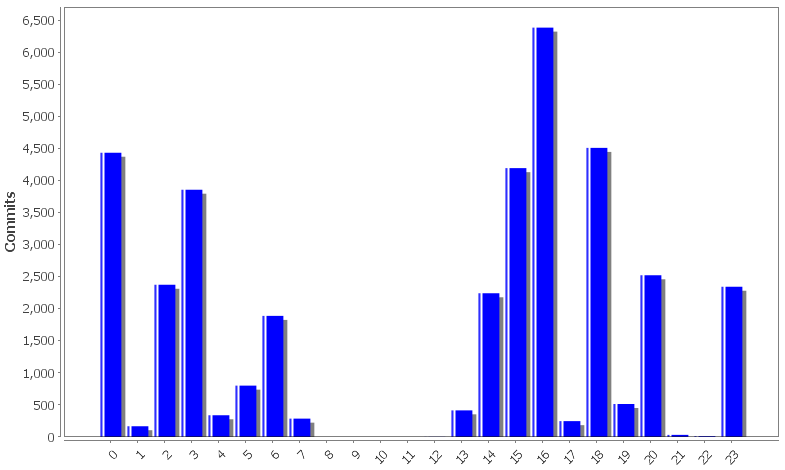
\includegraphics[scale=0.7]{pages/chapter4/figures/activity_time.png}
			\caption{Commit activity by hour of the day}
			\label{fig:activity_time}
		\end{figurehere}					
			
